\documentclass{article}

% content/resources/templates/preamble.tex
\usepackage[margin=0.6in]{geometry}
\author{Milav Dabgar}
\usepackage{amsmath,amssymb,amsthm}
\usepackage{booktabs}
\usepackage{multirow}
\usepackage{xcolor}
\usepackage{tcolorbox}
\tcbuselibrary{breakable,skins}
\usepackage[colorlinks=true,linkcolor=blue]{hyperref}
\usepackage{titlesec}
\usepackage{enumitem}
\usepackage{tikz}
\usepackage{pgfplots}
\usepackage{circuitikz}
\usepackage[version=4]{mhchem}
\usepackage{longtable}
\usepackage{array}
\usepackage{float}
\usepackage{caption}
\usepackage{listings}

\lstset{
  basicstyle=\small\ttfamily,
  breaklines=true,
  breakatwhitespace=false,
  postbreak=\mbox{\textcolor{red}{$\hookrightarrow$}\space},
  float=false,
  numbers=left,
  numberstyle=\tiny\color{gray},
  numbersep=10pt,
  xleftmargin=2em,
  keywordstyle=\color{blue},
  commentstyle=\color{green!60!black},
  stringstyle=\color{purple},
  backgroundcolor=\color{gray!5},
  showstringspaces=false,
  tabsize=2,
  captionpos=b,
  keepspaces=true,
  columns=flexible
}

\pgfplotsset{compat=1.18}
\usetikzlibrary{shapes,arrows,positioning,calc,patterns,decorations.pathmorphing,decorations.markings,arrows.meta}

% Color scheme
\definecolor{headcolor}{RGB}{0,102,204}
\definecolor{keycolor}{RGB}{220,20,60}
\definecolor{solutioncolor}{RGB}{34,139,34}
\definecolor{mnemoniccolor}{RGB}{148,0,211}
\definecolor{codecolor}{RGB}{0,0,100}

% Spacing
\setlength{\parskip}{3pt}
\setlist[itemize]{nosep}
\setlist[enumerate]{nosep}

% Title formatting
\titleformat{\section}{\Large\bfseries\color{headcolor}}{\thesection}{1em}{}
\titleformat{\subsection}{\large\bfseries\color{headcolor}}{\thesubsection}{1em}{}

% Pandoc tightlist compatibility
\providecommand{\tightlist}{%
  \setlength{\itemsep}{0pt}\setlength{\parskip}{0pt}}

% Pandoc longtable compatibility
\newcounter{none}
\def\thenone{}


% content/resources/templates/english-boxes.tex

% Custom environments
\newtcolorbox{solutionbox}{
 breakable,
 enhanced,
 colback=solutioncolor!5!white,
 colframe=solutioncolor!75!black,
 fonttitle=\bfseries,
 title=Solution
}

\newtcolorbox{solutionboxnobreak}{
 colback=solutioncolor!5!white,
 colframe=solutioncolor!75!black,
 fonttitle=\bfseries,
 title=Solution
}

\newtcolorbox{keyformula}{
 breakable,
 enhanced,
 colback=keycolor!5!white,
 colframe=keycolor!75!black,
 fonttitle=\bfseries,
 title=Key Formula
}

\newtcolorbox{mnemonicboxenv}{
 breakable,
 enhanced,
 colback=mnemoniccolor!5!white,
 colframe=mnemoniccolor!75!black,
 fonttitle=\bfseries,
 title=Mnemonic
}

\newcommand{\mnemonicbox}[1]{%
  \begin{mnemonicboxenv}
    #1
  \end{mnemonicboxenv}
}


% Custom commands for GTU solutions
% This file defines semantic commands for consistent formatting

% Question command with automatic formatting
\newcommand{\question}[2]{%
  \section*{Question #1}%
  \textbf{#2}%
}

% OR question variant
\newcommand{\questionor}[2]{%
  \section*{Question #1 OR}%
  \textbf{#2}%
}

% Proper table environment with caption
\newenvironment{answertable}[1]{%
  \begin{table}[htbp]
  \centering
  \caption{#1}
}{%
  \end{table}
}

% Proper figure environment for diagrams
\newenvironment{answerdiagram}[1]{%
  \begin{figure}[htbp]
  \centering
  \caption{#1}
}{%
  \end{figure}
}

% Semantic markup for key terms
\newcommand{\keyword}[1]{\textbf{#1}}
\newcommand{\code}[1]{\texttt{#1}}
\newcommand{\classname}[1]{\texttt{#1}}
\newcommand{\methodname}[1]{\texttt{#1}}

% Proper quotation marks
\newcommand{\mnemonic}[1]{``#1''}


\title{Object Oriented Programming With Java (4341602) - Summer 2023 Solution}
\date{July 15, 2023}

\begin{document}
\maketitle

\questionmarks{1(a)}{3}{Differentiate between Procedure-Oriented Programming (POP) and Object-Oriented Programming (OOP).}

\begin{solutionbox}
\begin{center}
\captionof{table}{POP vs OOP}
\begin{tabulary}{\linewidth}{|L|L|L|}
\hline
\textbf{Aspect} & \textbf{POP} & \textbf{OOP} \\ \hline
Focus & Functions/Procedures & Objects and Classes \\ \hline
Data Security & Less secure, global data & More secure, data encapsulation \\ \hline
Problem Solving & Top-down approach & Bottom-up approach \\ \hline
Code Reusability & Limited & High through inheritance \\ \hline
Examples & C, Pascal & Java, C++, Python \\ \hline
\end{tabulary}
\end{center}

\begin{itemize}
    \item \keyword{POP}: Program divided into functions, data flows between functions
    \item \keyword{OOP}: Program organized around objects that contain both data and methods
\end{itemize}
\end{solutionbox}

\begin{mnemonicbox}
\mnemonic{POP Functions, OOP Objects}
\end{mnemonicbox}

\questionmarks{1(b)}{4}{Explain Super keyword in inheritance with suitable example.}

\begin{solutionbox}
\textbf{Super keyword} is used to access parent class members from child class.

\begin{center}
\captionof{table}{Super keyword uses}
\begin{tabulary}{\linewidth}{|L|L|L|}
\hline
\textbf{Use} & \textbf{Purpose} & \textbf{Example} \\ \hline
\code{super()} & Call parent constructor & \code{super(name, age)} \\ \hline
\code{super.method()} & Call parent method & \code{super.display()} \\ \hline
\code{super.variable} & Access parent variable & \code{super.name} \\ \hline
\end{tabulary}
\end{center}

\begin{lstlisting}[language=Java,caption={Super Keyword Example}]
class Animal {
    String name = "Animal";
    void eat() { System.out.println("Animal eats"); }
}

class Dog extends Animal {
    String name = "Dog";
    void eat() {
        super.eat(); // calls parent method
        System.out.println("Dog eats bones");
    }
    void display() {
        System.out.println(super.name); // prints "Animal"
    }
}
\end{lstlisting}
\end{solutionbox}

\begin{mnemonicbox}
\mnemonic{Super calls Parent}
\end{mnemonicbox}

\questionmarks{1(c)}{7}{Define: Method Overriding. List out Rules for method overriding. Write a java program that implements method overriding.}

\begin{solutionbox}
\textbf{Method Overriding}: Child class provides specific implementation of parent class method with same signature.

\begin{center}
\captionof{table}{Method Overriding Rules}
\begin{tabulary}{\linewidth}{|L|L|}
\hline
\textbf{Rule} & \textbf{Description} \\ \hline
Same name & Method name must be identical \\ \hline
Same parameters & Parameter list must match exactly \\ \hline
IS-A relationship & Must have inheritance \\ \hline
Access modifier & Cannot reduce visibility \\ \hline
Return type & Must be same or covariant \\ \hline
\end{tabulary}
\end{center}

\begin{lstlisting}[language=Java,caption={Method Overriding Example}]
class Shape {
    void draw() {
        System.out.println("Drawing a shape");
    }
}

class Circle extends Shape {
    @Override
    void draw() {
        System.out.println("Drawing a circle");
    }
}

class Main {
    public static void main(String[] args) {
        Shape s = new Circle();
        s.draw(); // Output: Drawing a circle
    }
}
\end{lstlisting}
\end{solutionbox}

\begin{mnemonicbox}
\mnemonic{Override Same Signature}
\end{mnemonicbox}

\questionmarks{1(c OR)}{7}{Describe: Interface. Write a java program using interface to demonstrate multiple inheritance.}

\begin{solutionbox}
\textbf{Interface}: Blueprint containing abstract methods and constants. Classes implement interfaces to achieve multiple inheritance.

\begin{center}
\captionof{table}{Interface Features}
\begin{tabulary}{\linewidth}{|L|L|}
\hline
\textbf{Feature} & \textbf{Description} \\ \hline
Abstract methods & No implementation (before Java 8) \\ \hline
Constants & All variables are public static final \\ \hline
Multiple inheritance & Class can implement multiple interfaces \\ \hline
Default methods & Concrete methods (Java 8+) \\ \hline
\end{tabulary}
\end{center}

\begin{lstlisting}[language=Java,caption={Interface Example}]
interface Flyable {
    void fly();
}

interface Swimmable {
    void swim();
}

class Duck implements Flyable, Swimmable {
    public void fly() {
        System.out.println("Duck flies");
    }
    
    public void swim() {
        System.out.println("Duck swims");
    }
}

class Main {
    public static void main(String[] args) {
        Duck d = new Duck();
        d.fly();
        d.swim();
    }
}
\end{lstlisting}
\end{solutionbox}

\begin{mnemonicbox}
\mnemonic{Interface Multiple Implementation}
\end{mnemonicbox}

\questionmarks{2(a)}{3}{Explain the Java Program Structure with example.}

\begin{solutionbox}
\textbf{Java Program Structure} consists of package, imports, class declaration, and main method.

\begin{center}
\begin{tikzpicture}[node distance=1.5cm, auto]
    \node [gtu block] (pkg) {Package statement};
    \node [gtu block, below=0.5cm of pkg] (imp) {Import statements};
    \node [gtu block, below=0.5cm of imp] (cls) {Class declaration};
    \node [gtu block, below=0.5cm of cls] (vars) {Variables};
    \node [gtu block, below=0.5cm of vars] (meth) {Methods};
    
    \path [gtu arrow] (pkg) -- (imp);
    \path [gtu arrow] (imp) -- (cls);
    \path [gtu arrow] (cls) -- (vars);
    \path [gtu arrow] (vars) -- (meth);
\end{tikzpicture}
\captionof{figure}{Java Program Structure}
\end{center}

\begin{lstlisting}[language=Java,caption={Program Structure Example}]
package com.example;        // Package
import java.util.*;         // Import

public class HelloWorld {   // Class
    static int count = 0;   // Variable
    
    public static void main(String[] args) { // Main method
        System.out.println("Hello World");
    }
}
\end{lstlisting}
\end{solutionbox}

\begin{mnemonicbox}
\mnemonic{Package Import Class Main}
\end{mnemonicbox}

\questionmarks{2(b)}{4}{Explain static keyword with suitable example.}

\begin{solutionbox}
\textbf{Static keyword} belongs to class rather than instance. Memory allocated once.

\begin{center}
\captionof{table}{Static Uses}
\begin{tabulary}{\linewidth}{|L|L|L|}
\hline
\textbf{Type} & \textbf{Description} & \textbf{Example} \\ \hline
Static variable & Shared by all objects & \code{static int count} \\ \hline
Static method & Called without object & \code{static void display()} \\ \hline
Static block & Executes before main & \code{static \{ \}} \\ \hline
\end{tabulary}
\end{center}

\begin{lstlisting}[language=Java,caption={Static Keyword Example}]
class Student {
    static String college = "GTU";  // static variable
    String name;
    
    static void showCollege() {     // static method
        System.out.println(college);
    }
    
    static {                        // static block
        System.out.println("Static block executed");
    }
}

class Main {
    public static void main(String[] args) {
        Student.showCollege(); // No object needed
    }
}
\end{lstlisting}
\end{solutionbox}

\begin{mnemonicbox}
\mnemonic{Static Shared by Class}
\end{mnemonicbox}

\questionmarks{2(c)}{7}{Define: Constructor. List out types of it. Explain Parameterized and copy constructor with suitable example.}

\begin{solutionbox}
\textbf{Constructor}: Special method to initialize objects, same name as class, no return type.

\begin{center}
\captionof{table}{Constructor Types}
\begin{tabulary}{\linewidth}{|L|L|L|}
\hline
\textbf{Type} & \textbf{Description} & \textbf{Example} \\ \hline
Default & No parameters & \code{Student()} \\ \hline
Parameterized & With parameters & \code{Student(String name)} \\ \hline
Copy & Creates copy of object & \code{Student(Student s)} \\ \hline
\end{tabulary}
\end{center}

\begin{lstlisting}[language=Java,caption={Constructor Example}]
class Student {
    String name;
    int age;
    
    // Parameterized constructor
    Student(String n, int a) {
        name = n;
        age = a;
    }
    
    // Copy constructor
    Student(Student s) {
        name = s.name;
        age = s.age;
    }
    
    void display() {
        System.out.println(name + " " + age);
    }
}

class Main {
    public static void main(String[] args) {
        Student s1 = new Student("John", 20);  // Parameterized
        Student s2 = new Student(s1);          // Copy
        s1.display();
        s2.display();
    }
}
\end{lstlisting}
\end{solutionbox}

\begin{mnemonicbox}
\mnemonic{Constructor Initializes Objects}
\end{mnemonicbox}

\questionmarks{2(a OR)}{3}{Explain the Primitive Data Types and User Defined Data Types in java.}

\begin{solutionbox}
\textbf{Primitive Data Types}: Built-in types provided by Java language.
\textbf{User Defined Types}: Custom types created by programmer using classes.

\begin{center}
\captionof{table}{Data Types}
\begin{tabulary}{\linewidth}{|L|L|L|L|}
\hline
\textbf{Category} & \textbf{Types} & \textbf{Size} & \textbf{Example} \\ \hline
Primitive & byte, short, int, long & 1,2,4,8 bytes & \code{int x = 10;} \\ \hline
Primitive & float, double & 4,8 bytes & \code{double d = 3.14;} \\ \hline
Primitive & char, boolean & 2,1 bytes & \code{char c = 'A';} \\ \hline
User Defined & Class, Interface, Array & Variable & \code{Student s;} \\ \hline
\end{tabulary}
\end{center}

\begin{itemize}
    \item \keyword{Primitive}: Stored in stack, faster access
    \item \keyword{User Defined}: Stored in heap, complex operations
\end{itemize}
\end{solutionbox}

\begin{mnemonicbox}
\mnemonic{Primitive Built-in, User Custom}
\end{mnemonicbox}

\questionmarks{2(b OR)}{4}{Explain this keyword with suitable example.}

\begin{solutionbox}
\textbf{This keyword} refers to current object instance, used to distinguish between instance and local variables.

\begin{center}
\captionof{table}{This keyword uses}
\begin{tabulary}{\linewidth}{|L|L|L|}
\hline
\textbf{Use} & \textbf{Purpose} & \textbf{Example} \\ \hline
\code{this.variable} & Access instance variable & \code{this.name = name;} \\ \hline
\code{this.method()} & Call instance method & \code{this.display();} \\ \hline
\code{this()} & Call constructor & \code{this(name, age);} \\ \hline
\end{tabulary}
\end{center}

\begin{lstlisting}[language=Java,caption={This Keyword Example}]
class Student {
    String name;
    int age;
    
    Student(String name, int age) {
        this.name = name;    // this distinguishes
        this.age = age;      // instance from parameter
    }
    
    void setData(String name) {
        this.name = name;    // this refers to current object
    }
    
    void display() {
        System.out.println(this.name + " " + this.age);
    }
}
\end{lstlisting}
\end{solutionbox}

\begin{mnemonicbox}
\mnemonic{This Current Object}
\end{mnemonicbox}

\questionmarks{2(c OR)}{7}{Define Inheritance. List out types of it. Explain multilevel and hierarchical inheritance with suitable example.}

\begin{solutionbox}
\textbf{Inheritance}: Mechanism where child class acquires properties and methods of parent class.

\begin{center}
\captionof{table}{Inheritance Types}
\begin{tabulary}{\linewidth}{|L|L|L|}
\hline
\textbf{Type} & \textbf{Description} & \textbf{Structure} \\ \hline
Single & One parent, one child & A $\to$ B \\ \hline
Multilevel & Chain of inheritance & A $\to$ B $\to$ C \\ \hline
Hierarchical & One parent, multiple children & A $\to$ B, A $\to$ C \\ \hline
Multiple & Multiple parents (via interfaces) & B,C $\to$ A \\ \hline
\end{tabulary}
\end{center}

\begin{center}
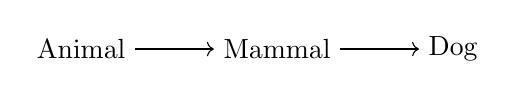
\begin{tikzpicture}[node distance=1.5cm]
    \node (A) {Animal};
    \node [right=1cm of A] (B) {Mammal};
    \node [right=1cm of B] (C) {Dog};
    \draw [->] (A) -- (B);
    \draw [->] (B) -- (C);
\end{tikzpicture}
\captionof{figure}{Multilevel Inheritance}
\end{center}

\begin{lstlisting}[language=Java,caption={Multilevel Inheritance Example}]
class Animal {
    void eat() { System.out.println("Animal eats"); }
}

class Mammal extends Animal {
    void breathe() { System.out.println("Mammal breathes"); }
}

class Dog extends Mammal {
    void bark() { System.out.println("Dog barks"); }
}
\end{lstlisting}

\begin{center}
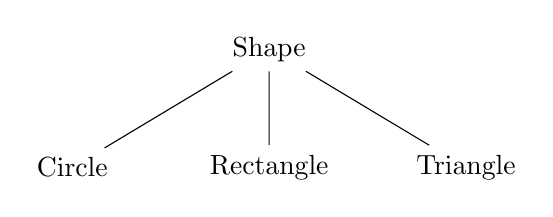
\begin{tikzpicture}[level distance=1.5cm, sibling distance=2.5cm]
  \node {Shape}
    child { node {Circle} }
    child { node {Rectangle} }
    child { node {Triangle} };
\end{tikzpicture}
\captionof{figure}{Hierarchical Inheritance}
\end{center}

\begin{lstlisting}[language=Java,caption={Hierarchical Inheritance Example}]
class Shape {
    void draw() { System.out.println("Drawing shape"); }
}

class Circle extends Shape {
    void drawCircle() { System.out.println("Drawing circle"); }
}

class Rectangle extends Shape {
    void drawRectangle() { System.out.println("Drawing rectangle"); }
}
\end{lstlisting}
\end{solutionbox}

\begin{mnemonicbox}
\mnemonic{Inheritance Shares Properties}
\end{mnemonicbox}

\questionmarks{3(a)}{3}{Explain Type Conversion and Casting in java.}

\begin{solutionbox}
\textbf{Type Conversion}: Converting one data type to another.
\textbf{Casting}: Explicit type conversion by programmer.

\begin{center}
\captionof{table}{Type Conversion}
\begin{tabulary}{\linewidth}{|L|L|L|}
\hline
\textbf{Type} & \textbf{Description} & \textbf{Example} \\ \hline
Implicit (Widening) & Automatic, smaller to larger & int to double \\ \hline
Explicit (Narrowing) & Manual, larger to smaller & double to int \\ \hline
\end{tabulary}
\end{center}

\begin{lstlisting}[language=Java,caption={Conversion vs Casting}]
// Implicit conversion
int i = 10;
double d = i;        // int to double (automatic)

// Explicit casting
double x = 10.5;
int y = (int) x;     // double to int (manual)

// String conversion
String s = String.valueOf(i);    // int to String
int z = Integer.parseInt("123"); // String to int
\end{lstlisting}
\end{solutionbox}

\begin{mnemonicbox}
\mnemonic{Implicit Auto, Explicit Manual}
\end{mnemonicbox}

\questionmarks{3(b)}{4}{Explain different visibility controls used in Java.}

\begin{solutionbox}
\textbf{Visibility Controls (Access Modifiers)}: Control access to classes, methods, and variables.

\begin{center}
\captionof{table}{Access Modifiers}
\begin{tabulary}{\linewidth}{|L|C|C|C|C|}
\hline
\textbf{Modifier} & \textbf{Same Class} & \textbf{Same Pkg} & \textbf{Subclass} & \textbf{Diff Pkg} \\ \hline
private & \checkmark & \times & \times & \times \\ \hline
default & \checkmark & \checkmark & \times & \times \\ \hline
protected & \checkmark & \checkmark & \checkmark & \times \\ \hline
public & \checkmark & \checkmark & \checkmark & \checkmark \\ \hline
\end{tabulary}
\end{center}

\begin{lstlisting}[language=Java,caption={Access Modifiers}]
class Example {
    private int x = 10;      // Only within class
    int y = 20;              // Package level
    protected int z = 30;    // Package + subclass
    public int w = 40;       // Everywhere
    
    private void method1() { }    // Private method
    public void method2() { }     // Public method
}
\end{lstlisting}
\end{solutionbox}

\begin{mnemonicbox}
\mnemonic{Private Package Protected Public}
\end{mnemonicbox}

\questionmarks{3(c)}{7}{Define: Thread. List different methods used to create Thread. Explain Thread life cycle in detail.}

\begin{solutionbox}
\textbf{Thread}: Lightweight subprocess that allows concurrent execution of multiple parts of program.

\begin{center}
\captionof{table}{Thread Creation Methods}
\begin{tabulary}{\linewidth}{|L|L|L|}
\hline
\textbf{Method} & \textbf{Description} & \textbf{Example} \\ \hline
Extending Thread & Inherit Thread class & \code{class MyThread extends Thread} \\ \hline
Implementing Runnable & Implement Runnable interface & \code{class MyTask implements Runnable} \\ \hline
\end{tabulary}
\end{center}

\begin{center}
\begin{tikzpicture}[node distance=1.8cm, auto]
    \node [gtu state] (new) {NEW};
    \node [gtu state, right=of new] (runnable) {RUNNABLE};
    \node [gtu state, right=of runnable] (running) {RUNNING};
    \node [gtu state, below=of running] (blocked) {BLOCKED};
    \node [gtu state, right=of running] (term) {TERMINATED};

    \path [gtu arrow] (new) -- (runnable);
    \path [gtu arrow] (runnable) -- node[font=\small] {CPU} (running);
    \path [gtu arrow] (running) edge [bend left] node[font=\small] {yield()} (runnable);
    \path [gtu arrow] (running) -- node[font=\small] {wait()} (blocked);
    \path [gtu arrow] (blocked) edge [bend left] node[font=\small] {notify()} (runnable);
    \path [gtu arrow] (running) -- (term);
\end{tikzpicture}
\captionof{figure}{Thread Life Cycle}
\end{center}

\begin{center}
\captionof{table}{Thread States}
\begin{tabulary}{\linewidth}{|L|L|}
\hline
\textbf{State} & \textbf{Description} \\ \hline
NEW & Thread created but not started \\ \hline
RUNNABLE & Ready to run, waiting for CPU \\ \hline
RUNNING & Currently executing \\ \hline
BLOCKED & Waiting for resource or sleep \\ \hline
TERMINATED & Execution completed \\ \hline
\end{tabulary}
\end{center}

\begin{lstlisting}[language=Java,caption={Thread Creation Example}]
// Method 1: Extending Thread
class MyThread extends Thread {
    public void run() {
        System.out.println("Thread running");
    }
}

// Method 2: Implementing Runnable
class MyTask implements Runnable {
    public void run() {
        System.out.println("Task running");
    }
}

class Main {
    public static void main(String[] args) {
        MyThread t1 = new MyThread();
        Thread t2 = new Thread(new MyTask());
        t1.start();
        t2.start();
    }
}
\end{lstlisting}
\end{solutionbox}

\begin{mnemonicbox}
\mnemonic{Thread Concurrent Execution}
\end{mnemonicbox}

\questionmarks{3(a OR)}{3}{Explain the purpose of JVM in java.}

\begin{solutionbox}
\textbf{JVM (Java Virtual Machine)}: Runtime environment that executes Java bytecode and provides platform independence.

\begin{center}
\captionof{table}{JVM Components}
\begin{tabulary}{\linewidth}{|L|L|}
\hline
\textbf{Component} & \textbf{Purpose} \\ \hline
Class Loader & Loads .class files into memory \\ \hline
Execution Engine & Executes bytecode \\ \hline
Memory Area & Manages heap and stack memory \\ \hline
Garbage Collector & Automatic memory management \\ \hline
\end{tabulary}
\end{center}

\begin{center}
\begin{tikzpicture}[node distance=1.5cm]
    \node [gtu block] (java) {Java Source (.java)};
    \node [gtu block, below=0.8cm of java] (comp) {Java Compiler (javac)};
    \node [gtu block, below=0.8cm of comp] (byte) {Bytecode (.class)};
    \node [gtu block, below=0.8cm of byte] (jvm) {JVM (Platform Specific)};
    
    \path [gtu arrow] (java) -- (comp);
    \path [gtu arrow] (comp) -- (byte);
    \path [gtu arrow] (byte) -- (jvm);
\end{tikzpicture}
\captionof{figure}{JVM Workflow}
\end{center}

\begin{itemize}
    \item \textbf{Platform Independence}: "Write Once, Run Anywhere"
    \item \textbf{Memory Management}: Automatic garbage collection
    \item \textbf{Security}: Bytecode verification
\end{itemize}
\end{solutionbox}

\begin{mnemonicbox}
\mnemonic{JVM Java Virtual Machine}
\end{mnemonicbox}

\questionmarks{3(b OR)}{4}{Define: Package. Write the steps to create a Package with suitable example.}

\begin{solutionbox}
\textbf{Package}: Collection of related classes and interfaces grouped together, providing namespace and access control.

\begin{center}
\captionof{table}{Package Benefits}
\begin{tabulary}{\linewidth}{|L|L|}
\hline
\textbf{Benefit} & \textbf{Description} \\ \hline
Namespace & Avoid name conflicts \\ \hline
Access Control & Better encapsulation \\ \hline
Organization & Logical grouping \\ \hline
Reusability & Easy to maintain \\ \hline
\end{tabulary}
\end{center}

\textbf{Steps to create Package:}
\begin{enumerate}
    \item \textbf{Declare package} at top of file
    \item \textbf{Create directory} structure matching package name
    \item \textbf{Compile} with package structure
    \item \textbf{Import} in other classes
\end{enumerate}

\begin{lstlisting}[language=Java,caption={Package Example}]
// File: com/company/utilities/Calculator.java
package com.company.utilities;

public class Calculator {
    public int add(int a, int b) {
        return a + b;
    }
}

// File: Main.java
import com.company.utilities.Calculator;

class Main {
    public static void main(String[] args) {
        Calculator calc = new Calculator();
        System.out.println(calc.add(5, 3));
    }
}
\end{lstlisting}

\begin{center}
\textbf{Directory Structure:}
\begin{verbatim}
com/
  company/
    utilities/
      Calculator.class
Main.class
\end{verbatim}
\end{center}
\end{solutionbox}

\begin{mnemonicbox}
\mnemonic{Package Groups Classes}
\end{mnemonicbox}

\questionmarks{3(c OR)}{7}{Explain Synchronization in Thread with suitable example.}

\begin{solutionbox}
\textbf{Synchronization}: Mechanism to control access to shared resources by multiple threads to avoid data inconsistency.

\begin{center}
\captionof{table}{Synchronization Types}
\begin{tabulary}{\linewidth}{|L|L|L|}
\hline
\textbf{Type} & \textbf{Description} & \textbf{Usage} \\ \hline
Synchronized method & Entire method locked & \code{synchronized void method()} \\ \hline
Synchronized block & Specific code block locked & \code{synchronized(object) \{ \}} \\ \hline
Static synchronization & Class level locking & \code{static synchronized void} \\ \hline
\end{tabulary}
\end{center}

\begin{center}
\begin{tikzpicture}[node distance=1.5cm, auto]
    \node [gtu state] (t1) {Thread 1};
    \node [gtu state, right=2cm of t1] (t2) {Thread 2};
    \node [gtu decision, below=1.5cm of t1] (lock) {Lock};
    \node [gtu block, below=1.5cm of lock] (res) {Shared Resource};
    \node [gtu state, below=1.5cm of res] (safe) {Safe Access};
    
    \path [gtu arrow] (t1) -- (lock);
    \path [gtu arrow] (t2) -- node {Wait} (lock);
    \path [gtu arrow] (lock) -- (res);
    \path [gtu arrow] (res) -- (safe);
\end{tikzpicture}
\captionof{figure}{Synchronization Mechanism}
\end{center}

\begin{lstlisting}[language=Java,caption={Synchronization Example}]
class Counter {
    private int count = 0;
    
    // Synchronized method
    public synchronized void increment() {
        count++;
    }
    
    // Synchronized block
    public void decrement() {
        synchronized(this) {
            count--;
        }
    }
    
    public int getCount() {
        return count;
    }
}

class CounterThread extends Thread {
    Counter counter;
    
    CounterThread(Counter c) {
        counter = c;
    }
    
    public void run() {
        for(int i = 0; i < 1000; i++) {
            counter.increment();
        }
    }
}

class Main {
    public static void main(String[] args) throws InterruptedException {
        Counter c = new Counter();
        CounterThread t1 = new CounterThread(c);
        CounterThread t2 = new CounterThread(c);
        
        t1.start();
        t2.start();
        
        t1.join();
        t2.join();
        
        System.out.println("Final count: " + c.getCount());
    }
}
\end{lstlisting}
\end{solutionbox}

\begin{mnemonicbox}
\mnemonic{Synchronization Prevents Race Conditions}
\end{mnemonicbox}

\questionmarks{4(a)}{3}{Differentiate between String class and StringBuffer class.}

\begin{solutionbox}
\begin{center}
\captionof{table}{String vs StringBuffer}
\begin{tabulary}{\linewidth}{|L|L|L|}
\hline
\textbf{Aspect} & \textbf{String} & \textbf{StringBuffer} \\ \hline
Mutability & Immutable (cannot change) & Mutable (can change) \\ \hline
Performance & Slower for concatenation & Faster for concatenation \\ \hline
Memory & Creates new object each time & Modifies existing object \\ \hline
Thread Safety & Thread safe & Thread safe \\ \hline
Methods & concat(), substring() & append(), insert(), delete() \\ \hline
\end{tabulary}
\end{center}

\begin{lstlisting}[language=Java,caption={String vs StringBuffer}]
// String - Immutable
String s1 = "Hello";
s1 = s1 + " World";  // Creates new String object

// StringBuffer - Mutable
StringBuffer sb = new StringBuffer("Hello");
sb.append(" World");  // Modifies existing object
\end{lstlisting}
\end{solutionbox}

\begin{mnemonicbox}
\mnemonic{String Immutable, StringBuffer Mutable}
\end{mnemonicbox}

\questionmarks{4(b)}{4}{Write a Java Program to find sum and average of 10 numbers of an array.}

\begin{solutionbox}
\begin{lstlisting}[language=Java,caption={Array Sum and Average}]
class ArraySum {
    public static void main(String[] args) {
        // Initialize array with 10 numbers
        int[] numbers = {10, 20, 30, 40, 50, 60, 70, 80, 90, 100};
        
        int sum = 0;
        
        // Calculate sum
        for(int i = 0; i < numbers.length; i++) {
            sum += numbers[i];
        }
        
        // Calculate average
        double average = (double) sum / numbers.length;
        
        // Display results
        System.out.println("Array elements: ");
        for(int num : numbers) {
            System.out.print(num + " ");
        }
        
        System.out.println("\nSum: " + sum);
        System.out.println("Average: " + average);
    }
}
\end{lstlisting}

\begin{center}
\textbf{Output:}
\begin{verbatim}
Array elements: 10 20 30 40 50 60 70 80 90 100
Sum: 550
Average: 55.0
\end{verbatim}
\end{center}

\textbf{Logic Steps:}
\begin{enumerate}
    \item Initialize array with 10 numbers
    \item Loop through array to calculate sum
    \item Calculate average = sum / length
    \item Display results
\end{enumerate}
\end{solutionbox}

\begin{mnemonicbox}
\mnemonic{Loop Sum Divide Average}
\end{mnemonicbox}

\questionmarks{4(c)}{7}{I) Explain abstract class with suitable example. II) Explain final class with suitable example.}

\begin{solutionbox}
\textbf{I) Abstract Class}: Class that cannot be instantiated, contains abstract methods that must be implemented by subclasses.

\begin{center}
\captionof{table}{Abstract Class Features}
\begin{tabulary}{\linewidth}{|L|L|}
\hline
\textbf{Feature} & \textbf{Description} \\ \hline
Cannot instantiate & No object creation \\ \hline
Abstract methods & Methods without implementation \\ \hline
Concrete methods & Methods with implementation \\ \hline
Inheritance & Subclasses must implement abstract methods \\ \hline
\end{tabulary}
\end{center}

\begin{lstlisting}[language=Java,caption={Abstract Class Example}]
abstract class Shape {
    String color;
    
    // Abstract method
    abstract void draw();
    
    // Concrete method
    void setColor(String c) {
        color = c;
    }
}

class Circle extends Shape {
    void draw() {
        System.out.println("Drawing Circle");
    }
}

class Main {
    public static void main(String[] args) {
        // Shape s = new Shape(); // Error: Cannot instantiate
        Circle c = new Circle();
        c.draw();
    }
}
\end{lstlisting}

\textbf{II) Final Class}: Class that cannot be extended (no inheritance allowed).

\begin{center}
\captionof{table}{Final Class Features}
\begin{tabulary}{\linewidth}{|L|L|}
\hline
\textbf{Feature} & \textbf{Description} \\ \hline
No inheritance & Cannot be extended \\ \hline
Security & Prevents modification \\ \hline
Performance & Better optimization \\ \hline
Examples & String, Integer, System \\ \hline
\end{tabulary}
\end{center}

\begin{lstlisting}[language=Java,caption={Final Class Example}]
final class FinalClass {
    void display() {
        System.out.println("This is final class");
    }
}

// class SubClass extends FinalClass { } // Error: Cannot extend

class Main {
    public static void main(String[] args) {
        FinalClass obj = new FinalClass();
        obj.display();
    }
}
\end{lstlisting}
\end{solutionbox}

\begin{mnemonicbox}
\mnemonic{Abstract Incomplete, Final Complete}
\end{mnemonicbox}

\questionmarks{4(a OR)}{3}{Explain Garbage Collection in Java.}

\begin{solutionbox}
\textbf{Garbage Collection}: Automatic memory management process that removes unused objects from heap memory.

\begin{center}
\captionof{table}{GC Benefits}
\begin{tabulary}{\linewidth}{|L|L|}
\hline
\textbf{Benefit} & \textbf{Description} \\ \hline
Automatic & No manual memory management \\ \hline
Memory leak prevention & Removes unreferenced objects \\ \hline
Performance & Optimizes memory usage \\ \hline
Safety & Prevents memory errors \\ \hline
\end{tabulary}
\end{center}

\begin{center}
\begin{tikzpicture}[node distance=1.5cm]
    \node [gtu block] (new) {Object created (new)};
    \node [gtu block, below=0.8cm of new] (use) {Object in use};
    \node [gtu block, below=0.8cm of use] (noref) {No references (Unreachable)};
    \node [gtu block, below=0.8cm of noref] (gc) {Garbage Collector removes};
    
    \path [gtu arrow] (new) -- (use);
    \path [gtu arrow] (use) -- (noref);
    \path [gtu arrow] (noref) -- (gc);
\end{tikzpicture}
\captionof{figure}{Garbage Collection Process}
\end{center}

\begin{itemize}
    \item \textbf{When occurs}: When heap memory is low or System.gc() called
    \item \textbf{Process}: Mark and Sweep algorithm
    \item \textbf{Cannot guarantee}: Exact timing of garbage collection
\end{itemize}
\end{solutionbox}

\begin{mnemonicbox}
\mnemonic{GC Automatic Memory Cleanup}
\end{mnemonicbox}

\questionmarks{4(b OR)}{4}{Write a Java program to handle user defined exception for 'Divide by Zero' error.}

\begin{solutionbox}
\begin{lstlisting}[language=Java,caption={User Defined Exception}]
// User defined exception class
class DivideByZeroException extends Exception {
    public DivideByZeroException(String message) {
        super(message);
    }
}

class Calculator {
    public static double divide(int a, int b) throws DivideByZeroException {
        if(b == 0) {
            throw new DivideByZeroException("Cannot divide by zero!");
        }
        return (double) a / b;
    }
}

class Main {
    public static void main(String[] args) {
        try {
            int num1 = 10;
            int num2 = 0;
            
            double result = Calculator.divide(num1, num2);
            System.out.println("Result: " + result);
            
        } catch(DivideByZeroException e) {
            System.out.println("Error: " + e.getMessage());
        }
    }
}
\end{lstlisting}

\begin{center}
\textbf{Output:}
\begin{verbatim}
Error: Cannot divide by zero!
\end{verbatim}
\end{center}
\end{solutionbox}

\begin{mnemonicbox}
\mnemonic{Custom Exception Handle Error}
\end{mnemonicbox}

\questionmarks{4(c OR)}{7}{Write a java program to demonstrate multiple try block and multiple catch block exception.}

\begin{solutionbox}
\begin{lstlisting}[language=Java,caption={Multiple Try-Catch Blocks}]
class MultipleExceptionDemo {
    public static void main(String[] args) {
        // First try block
        try {
            int[] arr = {1, 2, 3};
            System.out.println("Array element: " + arr[5]); // ArrayIndexOutOfBounds
        } 
        catch(ArrayIndexOutOfBoundsException e) {
            System.out.println("Array index error: " + e.getMessage());
        }
        catch(Exception e) {
            System.out.println("General exception: " + e.getMessage());
        }
        
        // Second try block
        try {
            String str = null;
            System.out.println("String length: " + str.length()); // NullPointer
        }
        catch(NullPointerException e) {
            System.out.println("Null pointer error: " + e.getMessage());
        }
        
        // Third try block with multiple catch
        try {
            int a = 10;
            int b = 0;
            int result = a / b;  // ArithmeticException
            
            String s = "abc";
            int num = Integer.parseInt(s);  // NumberFormatException
        }
        catch(ArithmeticException e) {
            System.out.println("Arithmetic error: " + e.getMessage());
        }
        catch(NumberFormatException e) {
            System.out.println("Number format error: " + e.getMessage());
        }
        catch(Exception e) {
            System.out.println("Other error: " + e.getMessage());
        }
        finally {
            System.out.println("Program completed");
        }
    }
}
\end{lstlisting}

\begin{center}
\textbf{Output:}
\begin{verbatim}
Array index error: Index 5 out of bounds for length 3
Null pointer error: null
Arithmetic error: / by zero
Program completed
\end{verbatim}
\end{center}
\end{solutionbox}

\begin{mnemonicbox}
\mnemonic{Multiple Try Multiple Catch}
\end{mnemonicbox}

\questionmarks{5(a)}{3}{Write a program in Java to create a file and perform write operation on this file.}

\begin{solutionbox}
\begin{lstlisting}[language=Java,caption={File Write Example}]
import java.io.*;

class FileWriteDemo {
    public static void main(String[] args) {
        try {
            // Create file
            File file = new File("demo.txt");
            
            // Create FileWriter object
            FileWriter writer = new FileWriter(file);
            
            // Write data to file
            writer.write("Hello World!\n");
            writer.write("This is Java file writing demo.\n");
            writer.write("File created successfully.");
            
            // Close the writer
            writer.close();
            
            System.out.println("File created and data written successfully!");
            
        } catch(IOException e) {
            System.out.println("Error: " + e.getMessage());
        }
    }
}
\end{lstlisting}
\end{solutionbox}

\begin{mnemonicbox}
\mnemonic{File Writer Write Close}
\end{mnemonicbox}

\questionmarks{5(b)}{4}{Explain throw and finally in Exception Handling with example.}

\begin{solutionbox}
\textbf{Throw}: Keyword used to explicitly throw an exception.
\textbf{Finally}: Block that always executes regardless of exception occurrence.

\begin{center}
\captionof{table}{Throw vs Finally}
\begin{tabulary}{\linewidth}{|L|L|L|}
\hline
\textbf{Keyword} & \textbf{Purpose} & \textbf{Usage} \\ \hline
throw & Explicitly throw exception & \code{throw new Exception()} \\ \hline
finally & Always execute cleanup code & \code{finally \{ \}} \\ \hline
\end{tabulary}
\end{center}

\begin{lstlisting}[language=Java,caption={Throw and Finally}]
class ThrowFinallyDemo {
    public static void checkAge(int age) throws Exception {
        if(age < 18) {
            throw new Exception("Age must be 18 or above");
        }
        System.out.println("Valid age: " + age);
    }
    
    public static void main(String[] args) {
        try {
            checkAge(15);  // Will throw exception
        }
        catch(Exception e) {
            System.out.println("Error: " + e.getMessage());
        }
        finally {
            System.out.println("Finally block always executes");
        }
    }
}
\end{lstlisting}
\end{solutionbox}

\begin{mnemonicbox}
\mnemonic{Throw Exception, Finally Always}
\end{mnemonicbox}

\questionmarks{5(c)}{7}{Describe: Polymorphism. Explain run time polymorphism with suitable example in java.}

\begin{solutionbox}
\textbf{Polymorphism}: One interface, multiple implementations. Object behaves differently based on its actual type.

\begin{center}
\captionof{table}{Polymorphism Types}
\begin{tabulary}{\linewidth}{|L|L|L|}
\hline
\textbf{Type} & \textbf{Description} & \textbf{When Decided} \\ \hline
Compile-time & Method overloading & At compilation \\ \hline
Run-time & Method overriding & At execution \\ \hline
\end{tabulary}
\end{center}

\begin{center}
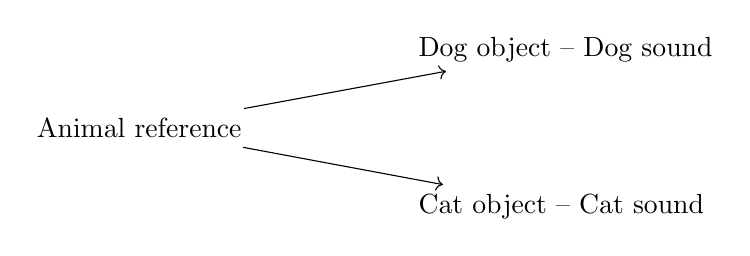
\begin{tikzpicture}[node distance=1.5cm, auto]
    \node (A) {Animal reference};
    \node [right=2cm of A, yshift=1cm] (B) {Dog object -- Dog sound};
    \node [right=2cm of A, yshift=-1cm] (C) {Cat object -- Cat sound};
    \draw [->] (A) -- (B);
    \draw [->] (A) -- (C);
\end{tikzpicture}
\captionof{figure}{Runtime Polymorphism}
\end{center}

\begin{lstlisting}[language=Java,caption={Runtime Polymorphism}]
class Animal {
    void makeSound() {
        System.out.println("Animal makes sound");
    }
}

class Dog extends Animal {
    @Override
    void makeSound() {
        System.out.println("Dog barks");
    }
}

class Cat extends Animal {
    @Override
    void makeSound() {
        System.out.println("Cat meows");
    }
}

class Main {
    public static void main(String[] args) {
        Animal animal1 = new Dog();  // Upcasting
        Animal animal2 = new Cat();  // Upcasting
        
        animal1.makeSound();  // Output: Dog barks
        animal2.makeSound();  // Output: Cat meows
        
        // Array of animals
        Animal[] animals = {new Dog(), new Cat(), new Dog()};
        for(Animal a : animals) {
            a.makeSound();  // Dynamic method dispatch
        }
    }
}
\end{lstlisting}
\end{solutionbox}

\begin{mnemonicbox}
\mnemonic{Polymorphism Many Forms Runtime}
\end{mnemonicbox}

\questionmarks{5(a OR)}{3}{Write a program in Java that read the content of a file byte by byte and copy it into another file.}

\begin{solutionbox}
\begin{lstlisting}[language=Java,caption={Byte Stream File Copy}]
import java.io.*;

class FileCopyDemo {
    public static void main(String[] args) {
        try {
            // Create input stream to read from source file
            FileInputStream input = new FileInputStream("source.txt");
            
            // Create output stream to write to destination file
            FileOutputStream output = new FileOutputStream("destination.txt");
            
            int byteData;
            
            // Read byte by byte and copy
            while((byteData = input.read()) != -1) {
                output.write(byteData);
            }
            
            // Close streams
            input.close();
            output.close();
            
            System.out.println("File copied successfully!");
            
        } catch(IOException e) {
            System.out.println("Error: " + e.getMessage());
        }
    }
}
\end{lstlisting}
\end{solutionbox}

\begin{mnemonicbox}
\mnemonic{Read Byte Write Byte}
\end{mnemonicbox}

\questionmarks{5(b OR)}{4}{Explain the different I/O Classes available with Java.}

\begin{solutionbox}
\begin{center}
\captionof{table}{Java I/O Classes}
\begin{tabulary}{\linewidth}{|L|L|L|}
\hline
\textbf{Class Type} & \textbf{Class Name} & \textbf{Purpose} \\ \hline
Byte Stream & FileInputStream & Read bytes from file \\ \hline
Byte Stream & FileOutputStream & Write bytes to file \\ \hline
Character Stream & FileReader & Read characters from file \\ \hline
Character Stream & FileWriter & Write characters to file \\ \hline
Buffered & BufferedReader & Efficient character reading \\ \hline
Buffered & BufferedWriter & Efficient character writing \\ \hline
\end{tabulary}
\end{center}

\begin{center}
\begin{tikzpicture}[node distance=1.2cm]
    \node [gtu block] (io) {Java I/O};
    \node [gtu block, below left=1cm of io] (byte) {Byte Stream};
    \node [gtu block, below right=1cm of io] (char) {Character Stream};
    
    \node [gtu block, below=0.5cm of byte] (fis) {FileInputStream};
    \node [gtu block, below=0.5cm of fis] (fos) {FileOutputStream};
    
    \node [gtu block, below=0.5cm of char] (fr) {FileReader};
    \node [gtu block, below=0.5cm of fr] (fw) {FileWriter};
    
    \path [gtu arrow] (io) -- (byte);
    \path [gtu arrow] (io) -- (char);
    \path [gtu arrow] (byte) -- (fis);
    \path [gtu arrow] (byte) -- (fos);
    \path [gtu arrow] (char) -- (fr);
    \path [gtu arrow] (char) -- (fw);
\end{tikzpicture}
\captionof{figure}{I/O Class Hierarchy}
\end{center}
\end{solutionbox}

\begin{mnemonicbox}
\mnemonic{Byte Character Buffered Streams}
\end{mnemonicbox}

\questionmarks{5(c OR)}{7}{Write a java program that executes two threads. One thread displays "Java Programming" every 3 seconds, and the other displays "Semester - 4th IT" every 6 seconds.}

\begin{solutionbox}
\begin{lstlisting}[language=Java,caption={Thread Timing Example}]
class JavaThread extends Thread {
    public void run() {
        try {
            while(true) {
                System.out.println("Java Programming");
                Thread.sleep(3000);  // Sleep for 3 seconds
            }
        } catch(InterruptedException e) {
            System.out.println("JavaThread interrupted");
        }
    }
}

class SemesterThread extends Thread {
    public void run() {
        try {
            while(true) {
                System.out.println("Semester - 4th IT");
                Thread.sleep(6000);  // Sleep for 6 seconds
            }
        } catch(InterruptedException e) {
            System.out.println("SemesterThread interrupted");
        }
    }
}

class Main {
    public static void main(String[] args) {
        // Create thread objects
        JavaThread javaThread = new JavaThread();
        SemesterThread semesterThread = new SemesterThread();
        
        // Start both threads
        javaThread.start();
        semesterThread.start();
        
        // Let threads run for 20 seconds then stop
        try {
            Thread.sleep(20000);
            javaThread.interrupt();
            semesterThread.interrupt();
        } catch(InterruptedException e) {
            System.out.println("Main thread interrupted");
        }
    }
}
\end{lstlisting}
\end{solutionbox}

\begin{mnemonicbox}
\mnemonic{Two Threads Different Timing}
\end{mnemonicbox}

\end{document}
